\documentclass{article}

\usepackage[utf8]{inputenc} 
\usepackage{enumitem}
\usepackage[left=2.5cm, right=2.5cm, top=2.5cm, bottom=2.5cm]{geometry}

% You may get an error here
% Some stackoverflow links that may be help you
% [Modifying settings.json in vscode to add shell escape flag to pdflatex in latex workshop] link: https://stackoverflow.com/questions/56743092/modifying-settings-json-in-vscode-to-add-shell-escape-flag-to-pdflatex-in-latex
% [How can I open Visual Studio Code's 'settings.json' file?] link: https://stackoverflow.com/questions/65908987/how-can-i-open-visual-studio-codes-settings-json-file
% [Pygmentize not installed error on Visual Studio Code] link: https://tex.stackexchange.com/questions/432459/pygmentize-not-installed-error-on-visual-studio-code
% Also note that pygmentize, which minted depends on uses python, so there may also be some issue with that (I lost some hours when first trying to set up minted :|)
\usepackage{minted} % colors for code

\usepackage{bussproofs} % proof trees
\usepackage{soul} % highlight text
\usepackage[x11names, dvipsnames]{xcolor} % choose color
\usepackage{amsthm} % for proof environment
\usepackage{hyperref} % Correct Section numbering, links
\usepackage{graphicx} % graphics
% math symbols
\usepackage{amssymb}
\usepackage{amsmath}
\usepackage{stmaryrd}
\usepackage{wasysym}

\setitemize{align=left, topsep = 5pt, parsep = 2pt}
\setenumerate{align=left}
\renewcommand*{\thesection}{\arabic{section}}

% Math shortcuts
\def\li{\rightarrow}
\def\fax{\forall x.}
\def\fay{\forall y.}
\def\faz{\forall z.}
\def\fan{\forall n. : Nat}
\def\exx{\exists x.}
\def\exy{\exists y.}
\def\exz{\exists z.}
\def\A{\mathcal{A}}
\def\B{\mathcal{B}}
\def\P{\mathcal{P}}
\def\tt{\texttt{tt}}
\def\ff{\texttt{ff}}
\def\nott{\texttt{not }}
\def\andt{\texttt{ and }}
\def\ort{\texttt{ or }}
\def\ift{\texttt{if }}
\def\thent{\texttt{ then }}
\def\elset{\texttt{ else }}
\def\endt{\texttt{ end}}
\def\skipt{\texttt{skip}}
\def\whilet{\texttt{while }}
\def\dot{\texttt{ do }}
\def\repeatt{\texttt{repeat }}
\def\untilt{\texttt{ until }}
\def\llb{\llbracket}
\def\rrb{\rrbracket}
\def\la{\langle}
\def\ra{\rangle}
\def\unt{\, \text{U} \,}
\def\nex{\bigcirc \,}
\def\evt{\lozenge  \,}
\def\alw{\square \,}

\title{Formal Methods and Functional Programming}
\author{Isabel Haas (isabel.haas@inf.ethz.ch)}
\date{Summer 2022}

\begin{document}
\maketitle

\begin{abstract}
This document should give an overview over the types of exercises in the FMFP course and how to solve them. 
It also contains parts of theory and an overview of Haskell. \\
There is no guarantee for correctness or completeness, please refer to the course material. \\
Main sources are the course material and material provided by the course TA
Max Schlegel on \\ \url{https://n.ethz.ch/~mschlegel/fmfp22/}
\end{abstract}

\thispagestyle{empty}
\tableofcontents

\newpage

\part*{Functional Programming}
\addcontentsline{toc}{part}{Functional Programming}
\setcounter{section}{0}
\renewcommand*{\theHsection}{chX.\the\value{section}}

\section{Haskell}
\textbf{Credits}: Big parts of this section are copied from/inspired by \url{https://n.ethz.ch/~mschlegel/fmfp22/}, hence credits go to Max
\setcounter{page}{1}
\subsection{Basics}
\begin{minted}{Haskell}
-- Basic function
-- Declaration, comparable to int mul(int a, int b){} in Java
mul :: Int -> Int -> Int 
mul a b = a + b -- Definition
-- function composition
f (g x) = f.g x
-- dollar sign:
f $ x = f x
f $ map g xs = f (map g xs) -- to avoid parentheses 
-- functions can also be arguments
filter :: (a->Bool) -> [a] -> [a] -- first arg: function taking a returning Bool
-- Pattern matching
fib :: Int -> Int
fib 0 = 0
fib 1 = 1
fib n = fib (n-1) + fib (n-2)
-- Guards
myAbs :: Int -> Int 
myAbs x
    | x < 0 = -x
    | otherwise = x
-- where 
f :: Int -> Int
f x = 1 + magic 
    where magic = sqrt x
-- let <def> in <expr> equal to <expr> where <def>
f :: Int -> Int
f x = (let magic = sqrt x in 1 + magic)
-- case expression (pattern matching)
case expression of pattern1 -> result1
                   pattern2 -> result2
div1byx :: Double -> Double
div1byx = case x of 0 -> 0.0
                    n -> 1/n
-- if else
if b then x else y -- returns either x or y
f x = if (prime x) then "PRIME" else "NOT" 
\end{minted}

\subsection{Lists}
\begin{minted}{Haskell}
[] -- empty list
x:xs -- first element is x, xs is rest of list
[a,b,c] -- syntactic sugar for a:b:c:[]
-- Basic pattern matching
f [] = 0
f (x:xs) = 2 + f xs
-- [1..x]
[1..4] -- [1,2,3,4]
[1,3..10] -- [1,3,5,7,9]
[5, 4..1] -- [5,4,3,2,1] 
[5..1] -- []
[1,2...] -- [1,2,...], used with lazy evaluation
-- List comprehensions
[f x | x <- list , guard_1, ..., guard_n]
[2*x | x <- [1..20], x `mod` 2 == 1] -- [2,6,10,..38]
[(l,r)| l <- "abc", r <- "xyz"] -- all comb. of characters in "abc" & "xyz"
-- Quick sort, very pretty
q (p:xs) = q [x | x <- xs, x <= p] ++ [p] ++ q [x | x <- xs, x > p]
\end{minted}

\subsection{Prelude functions}
\begin{minted}{Haskell}
-- Basics
head [1,2,3] -- 1 :: Int
tail [1,2,3] -- [2,3] :: [Int]
last [1,2,3] -- 3 :: Int
init [1,2,3] -- [1,2] :: [Int]
length [1,2,3] -- 3 :: Int
take 3 [1,2,3,4,5] -- [1,2,3] :: [Int]
drop 3 [1,2,3,4,5] -- [4,5] :: [Int]
reverse [1,2,3] -- [3,2,1] :: [Int]
maximum [1,2,3] -- 1 :: Int
minimum [1,2,3] -- 3 :: Int
sum [1,2,3,4] -- 10 :: Int
product [1,2,3,4] -- 24 :: Int
4 `elem` [1,2,3] -- False
-- More interesting
zip :: [a] -> [b] -> [(a,b)]
zip [1, 2] ['a', 'b'] == [(1,'a'),(2,'b')]
filter :: (a->Bool) -> [a] -> [a]
filter odd [1, 2, 3] -- [1,3]
map :: (a -> b) -> [a] -> [b]
map f [x1, x2, ..., xn] == [f x1, f x2, ..., f xn]
zipWith :: (a->b->c) -> [a] -> [b] -> [c]
zipWith f [x1,x2,x3..] [y1,y2,y3..] == [f x1 y1, f x2 y2, f x3 y3..]
-- right associative
foldr :: (a -> b -> b) -> b -> [a] -> b
foldr f z [] = z
foldr f z (x:xs) = f x (foldr f z xs)
foldr f z (a:b:c:[]) = f a (f b (f c (f z [])))
foldr (+) 0 [1..4] = 
-- left associative
foldl :: (a -> b -> b) -> b -> [a] -> b
foldr f z [] = z
foldl f z xs = foldl f z . toList
foldl f z (a:b:c:[]) = f (f a (f b)) c
-- returns longest prefix of elements satisfying p and corresponding remainder of list
span :: (a -> Bool) -> [a] -> ([a], [a]) -- span p xs
span (< 3) [1,2,3,4,1,2,3,4] -- ([1,2],[3,4,1,2,3,4])
curry :: ((a,b)->c) -> a -> b -> c
curry f a b = f (a,b)
uncurry :: (a->b->c) -> (a,b) -> c
uncurry f (x,y) = f x y
\end{minted}

\subsection{Algebraic data types}
Define new types
\begin{minted}{Haskell}
-- Structure: on the right side are value constructors
-- data type can have one of those different values
data keyword = constr1 | constr2 | ... | constrn
-- Option can be simple types
data Bool = False | True
-- New value constructors can be defined
-- Circle takes three floats as fields, rectangle 4
data Shape = Circle Float Float Float | Rectangle Float Float Float Float   
-- ghci> :t Circle
Circle :: Float -> Float -> Float -> Shape  
-- functions for data types
surface :: Shape -> Float  
surface (Circle _ _ r) = pi * r ^ 2  
surface (Rectangle x1 y1 x2 y2) = (abs $ x2 - x1) * (abs $ y2 - y1) 
-- has argument of type a or b
data myType a b = myConstr a | myOtherConstructor b
-- definitions can  be recursive
data myList a = Empty | Cons a (MyList a)
-- tree
data Tree t = Leaf | Node t (Tree t) (Tree t)

-- deriving keyword
-- typeclasses like Eq, Ord, Enum, Bounded, Show, Read can function as "interfaces"
-- Example: == and /= and can now be used to compare values
data Vector = Vector Int Int Int deriving (Eq, Show)

-- instance keyword
data TrafficLight = Red | Yellow | Green  
instance Eq TrafficLight where  
    Red == Red = True  
    Green == Green = True  
    Yellow == Yellow = True  
    _ == _ = False  
instance Show TrafficLight where  
    show Red = "Red light"  
    show Yellow = "Yellow light"  
    show Green = "Green light" 

-- fold for data types
-- data type:
data DType = C1 ... | C2 ... | ... | CN ...
-- fold
foldDType :: foldC1 -> foldC2 -> ... -> foldCN -> DType -> b
-- example
data Prop a = Var a | Not (Prop a) | And (Prop a) (Prop a) | Or (Prop a) (Prop a)
foldProp :: (a->b) -> (b->b) -> (b->b->b) -> (b->b->b) -> (Prop a) -> b
foldProp fVar fNot fAnd fOr prop  = go prop
    where 
        go (Var v) = fVar v
        go (Not v) = fNot (go v)
        go (And v w) = fAnd (go v) (go w) 
        go (Or v w) = fOr (go v) (go w)
\end{minted}  


\section{Evaluation strategies}
Lazy evaluation strategy of application \texttt{t1 t2}
\begin{enumerate}
    \item Evaluate \texttt{t1}
    \item The argument \texttt{t2} is substituted in \texttt{t1} without being evaluated
    \item No evaluation inside lambda abstractions. In other words, in an abstraction 
    \texttt{$\backslash$... -> f t}, then \texttt{f t} is not evaluated
\end{enumerate}
Eager evaluation strategy of application \texttt{t1 t2}
\begin{enumerate}
    \item Evaluate \texttt{t1}
    \item \texttt{t2} is evaluated prior to substitution in \texttt{t1}
    \item Evaluation is carried out inside lambda abstractions
\end{enumerate}

\subsection{Lazy evaluation in Haskell}
Haskell: Lazy Evaluation
\begin{itemize}
    \item argument only evaluated when no other steps possible
    \item left term is evaluated first
    \item argument made to fit pattern
\end{itemize}
\subsubsection{Sheet 1, Ex. 1}
\begin{minted}{Haskell}
fibLouis :: Int -> Int
fibLouis 0 = 1
fibLouis 1 = 1
fibLouis n = fibLouis (n - 1) + fibLouis (n - 2)
fibEva :: Int -> Int
fibEva n = fst (aux n) where 
    aux 0 = (0, 1)
    aux n = next (aux (n - 1))
    next (a, b) = (b, a + b)
\end{minted}
\textbf{Lazy Evaluation of fibLouis 4}
\begin{verbatim}
fibLouis 4 =
fibLouis (4-1) + fibLouis (4-2) =
-- most left term is evaluated first
fibLouis 3 + fibLouis (4-2) =
(fibLouis (3-1) + fibLouis (3-2)) + fibLouis (4-2) 
...
((fibLouis 1 + fibLouis (2-2)) + fibLouis (3-2)) + fibLouis (4-2) =
((1 + fibLouis (2-2)) + fibLouis (3-2)) + fibLouis (4-2) =
...
2 + fibLouis 2 =
2 + (fibLouis (2-1) + fibLouis (2-2))
... = 3
\end{verbatim}
\textbf{Lazy Evaluation of fibEva 4}
\begin{verbatim}
fibEva 4 =
fst (aux 4) =
fst (next (aux (4-1))) =
fst (next (aux 3)) =
fst (next (next (aux (3-1)))) =
fst (next (next (aux 2))) =
...
fst (next (next (next (next (0, 1))))) =
fst (next (next (next (1, 0+1)))) =
fst (next (next (0+1, 1+(0+1)))) =
fst (next (1+(0+1), (0+1)+(1+(0+1)))) 
...
-- pattern (0+1) is repeated
fst ((0+1)+(1+(0+1)), (1+(0+1))+((0+1)+(1+(0+1)))) =
(0+1)+(1+(0+1)) =
1 + (1 + 1) =
3
\end{verbatim}

\section{Natural Deduction}
\subsection{Parenthesizing formulas} 
\begin{itemize}
    \item $\land$ binds stronger than $\lor$ stronger than $\li$
    \item $\li$ associates to right; $\land$ and $\lor$ to the left
    \item Negation binds stronger than binary operators 
    \item Quantifiers extend to the right as far as possible: end of line or )
\end{itemize}
\begin{tabular}{l l}
    $p \lor q \land \lnot r \li p \lor q$ & $(p \lor (q \land (\lnot r))) \li (p \lor q)$ \\
    $p \li q \lor p \li r$ & $p \li ((q \lor p) \li r$) \\
    $p \land \fax q(x) \lor r$ & $p \land (\fax (q(x) \lor r))$ \\
    $\lnot \fax p(x) \land \fax q(x) \land r(x) \land s$ &  $\lnot( \fax (p(x) \land (\fax ((q(x) \land r(x)) \land s))))$
\end{tabular} 
\subsection{Natural Deduction without quantifiers}
If you cannot continue, try to add assumptions by using $\lor E$
\subsubsection{Example}
\textbf{Exercise}: $P = (\lnot A) \land (A \lor B) \li B$ is a tautology \\
First step: Parenthesizing $\Rightarrow$ $P \equiv ((\lnot A) \land (A \lor B)) \li B$ \\
Let $\Gamma \equiv (\lnot A) \land (A \lor B)$

\begin{prooftree}
    \def\ScoreOverhang{1pt}\def\ScoreOverhang{1pt}

    \AxiomC{}
    \RightLabel{$ax$}
    \UnaryInfC{$\Gamma, A \vdash (\lnot A) \land (A \lor B)$}
    \RightLabel{$\land ER$}
    \UnaryInfC{$\Gamma \vdash A \lor B$}
        \AxiomC{}
        \RightLabel{$ax$}
        \UnaryInfC{$\Gamma, A \vdash A$}

        \AxiomC{}
        \RightLabel{$ax$}
        \UnaryInfC{$\Gamma, A \vdash (\lnot A) \land (A \lor B)$}
        \RightLabel{$\land EL$}
        \UnaryInfC{$\Gamma, A \vdash \lnot A$}

        \RightLabel{$\lnot E$}
        \BinaryInfC{$\Gamma, A \vdash B$}
            \AxiomC{}
            \RightLabel{$ax$}
            \UnaryInfC{$\Gamma, B \vdash B$}
        \RightLabel{$\lor E$}
        \TrinaryInfC{$\Gamma \vdash B$}
        \RightLabel{$\li I$}
        \UnaryInfC{ $\vdash (\lnot A) \land (A \lor B) \li B$}
\end{prooftree}

\subsection{Natural Deduction with quantifiers}
If you cannot continue, try to add assumptions by using $\exists E$ \\
Always check side conditions
\subsubsection{Sheet 2, Ex. 3b}
\textbf{Exercise}: Proof $(\exx P \land Q) \li ((\exx P) \lor (\exx Q)) $ \\
Let $\Gamma \equiv \exx P \land Q, P \land Q$
\begin{prooftree}
    \def\ScoreOverhang{1pt}\def\ScoreOverhang{1pt}

    \AxiomC{}
    \RightLabel{$ax$}
    \UnaryInfC{$(\exx P \land Q) \vdash (\exx P \land Q)$}
        \AxiomC{}
        \RightLabel{$ax$}
        \UnaryInfC{$\Gamma \vdash P \land Q$}
        \RightLabel{$\land EL$}
        \UnaryInfC{$\Gamma \vdash P$}
        \RightLabel{$\exists I$}
        \UnaryInfC{$\Gamma \vdash \exx P$}

        \AxiomC{}
        \RightLabel{$ax$}
        \UnaryInfC{$\Gamma \vdash P \land Q$}
        \RightLabel{$\land ER$}
        \UnaryInfC{$\Gamma \vdash Q$}
        \RightLabel{$\exists I$}
        \UnaryInfC{$\Gamma \vdash \exx Q$}

        \RightLabel{$\land I$}
        \BinaryInfC{$\Gamma \vdash (\exx P) \land (\exx Q)$}
    \RightLabel{$\exists E ^{**}$}
    \BinaryInfC{$(\exx P \land Q) \vdash (\exx P) \land (\exx Q)$}
    \RightLabel{$\li I$}
    \UnaryInfC{$\vdash (\exx P \land Q) \li ((\exx P) \land (\exx Q))$}
\end{prooftree}

** side condition OK: x not free in $\exx P \land Q$ nor $(\exx P) \lor (\exx Q)$

\section{Binding and $\alpha$-conversion}
\textbf{Bound}: Each occurrence of a variable is bound or free:
A variable occurrence x in a formula A is \textbf{bound} if x occurs within a sub formula B of A of the form $\exx B$ or $\fax B$. \\
\textbf{Alpha-conversion}: bound variables can be renamed to names not yet used \\
\textbf{Examples} \\
\begin{tabular}{l l c}
     & & $\alpha$-convertible \\
    $\fax \exy p(x,y)$ & $\fay \exx p(y,x)$ & yes \\
    $\exz \fay p(z, f(y))$ &  $\exy \fay p(y, f(y))$ & no \\
    $(\fax p(x)) \lor (\exx q(x))$ & $(\faz p(z)) \lor (\exy q(y))$ & yes \\
    $p(x) \li \fax p(x)$ & $p(y) \li \fay p(y)$ & no \\
\end{tabular}

\section{Induction}
For proofs with \texttt{[]}, \texttt{0}. \texttt{Leaf} or similar, you may first have to proof a generalised statement with induction and then simply plug in your values.
\subsection{Induction on natural numbers}
Induction scheme:
\begin{prooftree}
    \AxiomC{$\Gamma \vdash P[n \mapsto 0]$}
    \AxiomC{$\Gamma, P[n \mapsto m] \vdash  P[n \mapsto m+1]$}
    \RightLabel{$m$ not free in P}
    \BinaryInfC{$\Gamma \vdash \forall n : Nat. P$}
\end{prooftree}

\subsubsection{Sheet 3, Ex. 1b}
(Important parts/"framework" of proof) \\
\textbf{Lemma}: $\fan$ \texttt{aux n = (fibLouis n, fibLouis (n+1))}
\begin{proof}
    Let \texttt{P:=}(aux n = (fibLouis n, fibLouis (n+1)))\\
    \textbf{Base case}. Show \texttt{P[n $\mapsto$ 0]} 
    \begin{minted}{Haskell}
    aux 0 = ...
        = (fibLouis 0, fibLouis (0+1))
    \end{minted}
    \textbf{Step case}: Let \texttt{m:Nat} be arbitrary. \\
    \textbf{I.H.}: \texttt{P[n $\mapsto$ m]} \\
    Show \texttt{P[n $\mapsto$ (m+1)]}. \\
    Assume \texttt{aux m = (fibLouis m, fibLouis (m+1))}
    \begin{minted}{Haskell}
    aux (m+1) = ...
            = (fibLouis (m+1), fibLouis ((m+1)+1)) 
    \end{minted}
\end{proof}

\subsection{Induction on lists}

Induction scheme:
\begin{prooftree}
    \AxiomC{$\Gamma \vdash P[xs \mapsto []]$}
    \AxiomC{$\Gamma, P[xs \mapsto ys] \vdash P[xs \mapsto (y:ys)]$}
    \RightLabel{$y, ys$ not free in P}
    \BinaryInfC{$\Gamma \vdash \forall xs :: [a]. P$}
\end{prooftree}

\subsubsection{Sheet 3, Ex. 2b}
(Important parts/"framework" of proof) \\
\textbf{Lemma}: \texttt{foldr (:) [] xs = xs}
\begin{proof}
    Let \texttt{P:= (foldr (:) [] xs = xs)}. \\
    We prove by induction over lists that $\forall xs::[a].$ \texttt{P} holds. \\
    \textbf{Base case}. Show \texttt{P[xs $\mapsto$ []]} 
    \begin{minted}{Haskell}
    foldr (:) [] [] = [] 
    \end{minted}
    \textbf{Step case}: Let \texttt{y::a, ys::[a]} be arbitrary. \\
    \textbf{I.H}.: \texttt{P[xs $\mapsto$ ys]}\\
    Show \texttt{P[xs $\mapsto$ (y:ys)]} \\
    Assume \texttt{foldr (:) [] ys = ys} % and we show that \texttt{foldr (:) [] (y:ys) = y:ys}
    \begin{minted}{Haskell}
    foldr (:) [] (y:ys) = 
        = ...
        = (y:ys)
    \end{minted}
\end{proof}
\subsubsection{Sheet 4, Ex. 1}
(Important parts/"framework" of proof) \\
\textbf{Lemma}: \texttt{rev (xs ++ rev ys) = ys ++ rev xs}
\begin{proof}
    Let \texttt{P' := rev (xs ++ rev ys') = ys' ++ rev xs}. 
    We show that $\forall$ \texttt{ys'.}$\forall$ \texttt{xs.}. \\
    Fix an arbitrary \texttt{ys} and let \texttt{P := [ys' $\mapsto$ ys]}.
    We show that $\forall$\texttt{xs P.} \\
    (This implies $\forall$\texttt{ys'.}$\forall$\texttt{xs.P'}) \\
    \textbf{Base case}: We show \texttt{P[xs $\mapsto$ []]} 
    \begin{minted}{Haskell}
    rev ([] ++ rev ys) = ...
        = ys ++ rev []
    \end{minted}
    \textbf{Step case}: Let \texttt{z::a, zs::[a]} be arbitrary. \\
    Fix arbitrary \texttt{y::a}, \texttt{ys::[a]}. \\
    \textbf{I.H.}: \texttt{ rev (zs ++ rev ys) = ys ++ rev zs}  \\
    We show \texttt{ P[xs $\mapsto$ (z:zs)]}.
    \begin{minted}{Haskell}
    rev ((z:zs) ++ rev ys)
        = ...
        = ys ++ rev (z:zs)
    \end{minted}
\end{proof}

\subsection{Induction on Trees}
\begin{minted}{Haskell}
data Tree t = Leaf | Node t (Tree t) (Tree t)
\end{minted}

Induction scheme:
\begin{prooftree}
    \AxiomC{$\Gamma \vdash P[x \mapsto \text{Leaf} ]$}
    \AxiomC{$\Gamma, P[x \mapsto l], P[x \mapsto r] \vdash P[x \mapsto \text{Node } a \, l \, r]$}
    \RightLabel{$a,l,r$ not free in P}
    \BinaryInfC{$\Gamma \vdash \forall xs :: \text{Tree } t. P$}
\end{prooftree}

\subsubsection{Sheet 6, Ex. 1}
(Important parts/"framework" of proof) 
\begin{minted}{Haskell}
mapTree f Leaf = Leaf
mapTree f (Node x t1 t2) = Node (f x) (mapTree f t1) (mapTree f t2) 
\end{minted}  
For arbitrary \mintinline{Haskell}{f :: a -> b} and \mintinline{Haskell}{g :: b -> c} \\
$\forall$\texttt{t :: Tree a. mapTree g (mapTree f t) = mapTree (g . f) t}

\begin{proof}
    Let \mintinline{Haskell}{f :: a -> b} and \mintinline{Haskell}{g :: b -> c} be arbitrary functions. \\
    Let \texttt{P := mapTree g (mapTree f t) = mapTree (g . f) t}, and we prove by induction that 
    $\forall$\texttt{t :: (Tree a).P} \\
    \textbf{Base Case}: Show \texttt{P[t $\mapsto$ Leaf]} 
    \begin{minted}{Haskell}
        mapTree g (mapTree f Leaf) = ..
                =  mapTree (g . f) Leaf
    \end{minted}
    \textbf{Step case}: 
    Let \texttt{x::a, l::Tree a, r::Tree a} be arbitrary. \\
    I.H.1: \texttt{P[t $\mapsto$ l]} \\
    I.H.2: \texttt{P[t $\mapsto$ r]} \\
    We show \texttt{P[t $\mapsto$ Node x l r]} 
    \begin{minted}{Haskell}
        mapTree g (mapTree f (Node x l r)) = ..
                =  mapTree (g . f) (Node x l r)
    \end{minted}
\end{proof}



\section{Types and typing inference}
\texttt{f :: a -> b -> c -> d}:
\begin{itemize}
    \item same as \texttt{f :: a -> (b -> (c -> d))} (parentheses are right associative) 
    \item \texttt{f x y z} implies \texttt{x::a, y::b, z::c} 
    \item f.e. \texttt{f x :: b -> c -> d}
\end{itemize}
\subsection{Types}
\begin{itemize}
    \item Detect function applications, f.e. \texttt{f x} $\Rightarrow$ \texttt{f::a->b, x::a}
    \item Detect prelude functions such as map, filter, foldr etc.
    \item "Match" types of different function, f.e. \texttt{f :: (a->b) -> [a] -> b} for  \texttt{f x} $\Rightarrow$ \texttt{x :: (a->b)}
    \item Don't forget things like \texttt{Num a, Eq b => ...}
\end{itemize}
% \textbf{Example} \\
% \mintinline{Haskell}{\x y -> (fst x) + y}
% \mintinline{Haskell}{(+) :: (Num a => a -> a -> a)} and \mintinline{Haskell}{fst :: (a,b) -> a} \\
% $\Rightarrow$ \mintinline{Haskell}{y :: (Num a) => a}, \mintinline{Haskell}{(fst x) ::  (Num a) => a} and
% \mintinline{Haskell}{x :: (c,b)} \\
% $\Rightarrow$ \mintinline{Haskell}{\x y -> (fst x) + y :: Num a => (a,b) -> a -> a}
\subsubsection{Sheet 5}
\textbf{1a} \verb|\x y z -> (x y) z|
\begin{enumerate}
    \item Three arguments, one return value
    \item \verb|(x y) :: a -> b| and \verb|z :: a|
    \item \verb|x :: c -> (a->b)| and \verb|y :: c|
    \item \verb|\x y z -> (x y) z :: (c -> a -> b) -> c -> a -> b|
\end{enumerate}
\textbf{2a.4} \texttt{(.).(.)} (the end boss)
\begin{enumerate}
    \item \texttt{(.) :: (b->c) -> (a->b) -> a -> c}
    \item Rewrite: \texttt{\textcolor{Red}{(.)}\textcolor{Cyan}{.}\textcolor{Green}{(.)} 
    = \textcolor{Cyan}{.}\textcolor{Red}{(.)}\textcolor{Green}{(.)} 
    = \textcolor{Cyan}{f} \textcolor{Red}{g} \textcolor{Green}{h}}
    \item Definition of \texttt{(.)}: \\
    \texttt{f :: (b->c) -> ((a->b) -> a -> c)} \\
    \texttt{g :: (n->o) -> ((m->n) -> m -> o)} \\
    \texttt{h :: (q->r) -> ((p->q) -> p -> r)} 
    \item \texttt{g} is first argument of \texttt{f}: \\
    \texttt{g :: b -> c} \\
    $\Rightarrow$ \texttt{b = n -> o} (I) and
    \texttt{c = (m->n) -> m -> o} (II)
    \item \texttt{h} is first argument of \texttt{f g}:\\
    \texttt{f g :: (a->b) -> a -> c}   \\
    $\Rightarrow$ \texttt{h :: a -> b}  \\
    $\Rightarrow$ \texttt{a = q -> r} (III)\\
    \texttt{b = (p->q) -> p -> r} (IV)
    \item (I) and (IV) $\Rightarrow$ 
    \texttt{n = p -> q} (V) and \texttt{o = p -> r}
    \item After "taking" two arguments, we have the following type \\
    \texttt{f g h :: a -> c} \\
    \texttt{= (q->r) -> (m->n) -> m -> o} \\
    \texttt{= (q->r) -> (m->p->q) -> m -> p -> r }
\end{enumerate}
\subsection{Typing proof and inference}
Solving type inference constraints
\begin{enumerate}
    \item Remove trivial equations like $t = t$
    % \item Merge equations $\{x=s, x =t\}$ into $\{s=t\}$ (if x doesn't appear in other equations)
    \item Transform equations of form $\{f(s_0, ..., s_k)=g(t_0, ..., s_m)\}$ into $\{s_0 = t_0, ..., s_k = t_k\}$ if
    $f=g$ and $k=m$, else there is no solution
    \item Substitute one equation into the others 
\end{enumerate}
\subsubsection{Sheet 5, Ex. 3}
\textbf{a} Proof $\lambda$\texttt{x.(x 1 True, x 0) :: (Int -> Bool -> a) -> (a, Bool -> a)}:\\
Try to match left and right side with typing rule and apply it, should be straight forward \\
\textbf{b} Infer the type of ($\lambda$\texttt{x.}$\lambda$\texttt{y.(y (iszero (y x)))) True}
\begin{prooftree}
    \def\ScoreOverhang{1pt}\def\ScoreOverhang{1pt}
    \AxiomC{}
    \RightLabel{$Var^1$}
    \UnaryInfC{$x : \tau_1, y : \tau_2 \vdash y :: \tau_4 \li \tau_3$}
    \AxiomC{$\mathbf{T_2}$}
    \RightLabel{$App$}
    \BinaryInfC{$x : \tau_1, y : \tau_2\vdash y \; (\mathbf{iszero}\; (y \; x)) :: \tau_3$ }
    \RightLabel{$Abs^1$}
    \UnaryInfC{$ x : \tau_1 \vdash \lambda y. (y \; (\mathbf{iszero}\; (y \; x))) :: \tau_0$}
    \RightLabel{$Abs$}
    \UnaryInfC{$\vdash \lambda x. \lambda y. (y \; (\mathbf{iszero}\; (y \; x))) :: \tau_1 \li \tau_0$}
        \AxiomC{}
        \RightLabel{$True^1$}
        \UnaryInfC{$\vdash True :: \tau_1$}
    \RightLabel{$App$}
    
    \BinaryInfC{ $\vdash (\lambda x. \lambda y. (y \; (\mathbf{iszero} \; (y \; x)))) \; True :: \tau_0$ }
\end{prooftree}
T$_2$:
\begin{prooftree}
    \AxiomC{}
    \RightLabel{$Var^2$}
    \UnaryInfC{$x : \tau_1, y : \tau_2\vdash y :: \tau_5 \li Int$}
    \AxiomC{}
    \RightLabel{$Var^3$}
    \UnaryInfC{$x : \tau_1, y : \tau_2\vdash x :: \tau_5$}
    \RightLabel{$App$}
    \BinaryInfC{$x : \tau_1, y : \tau_2 \vdash  y \; x :: Int$}
    \RightLabel{$iszero^1$}
    \UnaryInfC{$x : \tau_1, y : \tau_2\vdash \mathbf{iszero}\; (y \; x) :: \tau_4$}
    
\end{prooftree}

Finding out $\tau_0$: \\ \\
\begin{tabular}{l | l | l | l }
    $\tau_0 = \tau_2 \li \tau_3$ ($Abs^1$) & $\tau_0 = \tau_2 \li \tau_3$ & $\tau_0 = \tau_2 \li \tau_3$
    &  $\tau_0 = (Bool \li Int) \li \tau_3$\\

    $\tau_2 = \tau_4 \li \tau_3$ ($Var^1$) & $\tau_2 = \tau_4 \li \tau_3$ & $\tau_2 = \tau_4 \li \tau_3$
    & $Bool \li Int=\tau_4 \li \tau_3$\\

    $\tau_4 = Bool$ ($iszero^1$)& $\tau_4 = Bool$ & $\tau_4 = Bool$
    & $\tau_4 = Bool$\\

    $\tau_2 = \tau_5 \li Int$ ($Var^2$)& $\tau_2 = \tau_5 \li Int$ & $\tau_2 = Bool \li Int$
    & $\tau_5 = Bool$\\

    $\tau_1 = \tau_5$ ($Var^3$)& $\tau_5 = Bool$ & $\tau_5 = Bool$
    & \\

    $\tau_1 = Bool$ ($True^1$)& & & \\ \hline
\end{tabular}
\\
\begin{tabular}{l | l}
    $\tau_0 = (Bool \li Int) \li \tau_3$ & $\tau_0 = (Bool \li Int) \li Int$\\
    $\tau_3 = Int$ &  $\tau_3 = Int$\\
    $\tau_4 = Bool$ & $\tau_4 = Bool$\\
    $\tau_5 = Bool$ &  $\tau_5 = Bool$\\
\end{tabular}
\\ \\
\textbf{d} Infer type of \texttt{iszero(fst (3+5))}
\begin{prooftree}
    \AxiomC{}
    \RightLabel{$Int$}
    \UnaryInfC{$\vdash 3 :: Int$}
    \AxiomC{}
    \RightLabel{$Int$}
    \UnaryInfC{$\vdash 5 :: Int$}
    \RightLabel{$BinOp$}
    \BinaryInfC{$\vdash(3+5) :: (Int, \tau_1)$}
    \RightLabel{$fst$}
    \UnaryInfC{$\vdash \mathbf{fst} (3+5) :: Int$}
    \RightLabel{$iszero$}
    \UnaryInfC{$\vdash \mathbf{iszero}(\mathbf{fst} (3+5)) :: \tau_0$}
\end{prooftree}
Collected type constraints: $\tau_0 = Bool$ from $iszero$, $(Int = (Int, \tau_1))$ from $BinOp$, 
second constraint does not unify, meaning this doesn't type

\newpage
\part*{Formal Methods}
\addcontentsline{toc}{part}{Formal Methods}
\setcounter{section}{0}
\renewcommand*{\theHsection}{chY.\the\value{section}}

\section{Introduction to language semantics}
\subsection{States}
\textbf{State as a function}: 
$$\text{State: Var} \li \text{Val}$$ 
\textbf{Zero state}: 
$$\sigma_{zero}(x)=0\text{ for all }x$$
\textbf{Updating states}: 
$$ (\sigma[y\mapsto v](x)) = \begin{cases}
v & \text{if } x \equiv y \\
\sigma(x) & x \not\equiv y \\
\end{cases}
$$
\textbf{Two states are equal}:
$$ \sigma_1 = \sigma_2 \Leftrightarrow \fax (\sigma_1(x) = \sigma_2(x))$$

\subsection{Semantics of arithmetic expression}
\textbf{Semantic function}:
$$ \A: \text{Aexp}\li \text{State} \li \text{Val}$$
\textbf{Mapping}
\begin{center}
\begin{tabular}{l l}
    $\A \llb x\rrb \sigma$ & $= \sigma(x)$ \\
    $\A \llb n\rrb \sigma$ & $= \mathcal{N}\llb n\rrb$ \\
    $\A \llb e_1 \, op \, e_2\rrb \sigma$ & $= \A\llb e_1\rrb \, \overline{op} \, \A\llb e_2\rrb$ 
\end{tabular}
\end{center}
with $\overline{op}$ the relation $\text{Val}\times\text{Val}$ corresponding to $op$

\subsection{Semantics of boolean expression}
\textbf{Semantic function}:
$$ \B: \text{Bexp}\li \text{State} \li \text{Val}$$
\textbf{Mapping}
\begin{center}
\begin{tabular}{l l}
    $\B \llb e_1 \, op \, e_2 \rrb \sigma$ & $=
    \begin{cases}
        \tt & \text{if } \A \llb e_1\rrb \sigma \, \overline{op} \, \A \llb e_2\rrb \sigma \\
        \ff & \text{otherwise}
    \end{cases}$ \\
    $\B \llb b_1 \ort b_2 \rrb \sigma$ & $=
    \begin{cases}
        \tt & \text{if } \B \llb b_1\rrb \sigma = \tt \text{ or } \B \llb b_2\rrb \sigma  = \tt\\
        \ff & \text{otherwise}
    \end{cases}$ \\
    $\B \llb b_1 \andt b_2 \rrb \sigma$ & $=
    \begin{cases}
        \tt & \text{if } \B \llb b_1\rrb \sigma  = \tt \text{ and } \B \llb b_2\rrb \sigma  = \tt\\
        \ff & \text{otherwise}
    \end{cases}$ \\
    $\B \llb \nott b \rrb \sigma$ & $=
    \begin{cases}
        \tt & \text{if } \B \llb b\rrb \sigma = \ff \\
        \ff & \text{otherwise}
    \end{cases}$ \\
\end{tabular}
\end{center}
with $\overline{op}$ the relation $\text{Val}\times\text{Val}$ corresponding to $op$

\subsection{Free variables}
\begin{center}
    \begin{tabular}{l l}
        $FV(e_1 \, op \, e_2)$ & $=FV(e_1) \cup FV(e_2)$ \\
        $FV(n)$ & $=\emptyset$ \\
        $FV(x)$ & $=\{x\}$ \\
        $FV(\nott b)$ & $=FV(b)$ \\
        $FV(b_1 \ort b_2)$ & $=FV(b_1) \cup FV(b_2)$ \\
        $FV(b_1 \andt b_2)$ & $=FV(b_1) \cup FV(b_2)$ \\
        $FV(\skipt)$ & $= \emptyset$ \\
        $FV(x:=e)$ & $= \{x\} \cup FV(e)$ \\
        $FV(s_1;s_2)$ & $= FV(s_1) \cup FV(e_2)$ \\
        $FV(\ift b \thent s_1 \elset s_2 \endt )$ & $= FV(b) \cup FV(s_1) \cup FV(s_2)$ \\
        $FV(\whilet b \dot s \endt)$ & $= FV(b) \cup FV(s)$ \\
    \end{tabular}
\end{center}

\subsection{Substitution}

\begin{center}
    \begin{tabular}{l l}
        $(e_1 \, op \, e_2)[x \mapsto e]$ & $\equiv (e_1[x\mapsto e])$ \\
        $n[x\mapsto e]$ & $\equiv n$\\
        $y[x\mapsto e]$ & $\equiv\begin{cases} e & \text{if } x \equiv y \\ y & \text{otherwise} \end{cases}$\\
        $(\nott b)[x\mapsto e]$ & $\nott (b[x\mapsto e])$ \\
        $(b_1 \ort b_2)[x\mapsto e]$ &  $(b_1[x\mapsto e] \ort b_2[x\mapsto e])$ \\
        $(b_1 \andt b_2)[x\mapsto e]$ &  $(b_1[x\mapsto e] \andt b_2[x\mapsto e])$ \\
    \end{tabular}
\end{center}

\textbf{Substitution Lemma}:
$$ \B \llb b [x \mapsto e]\rrb \sigma = \B \llb b\rrb (\sigma[x \mapsto \A \llb e \rrb \sigma])$$

\subsection{Structural induction on arithmetic and boolean expressions}
\subsubsection{Session sheet 10, Ex. 2}
Statement: $ \forall \sigma, e, e', x \, \A \llb e [x \mapsto e']\rrb \sigma = \A \llb e \rrb (\sigma[x \mapsto \A \llb e' \rrb \sigma])$
\begin{proof}
    Let $\sigma, x, e'$ be arbitrary. \\
    Let $P(e) \equiv (\A \llb e [x \mapsto e']\rrb \sigma = \A \llb e \rrb (\sigma[x \mapsto \A \llb e' \rrb \sigma]))$.\\
    We prove $\forall e. P(e)$ by strong structural induction on $e$. \\
    We want to show $P(e)$ for some arbitrary $e$ and assume $\forall e''  \sqsubset e \, P(e')$ (\textbf{I.H.})\\
    \textbf{Case} $e \equiv n$ for some numerical value n:\\
    \dots \\
    \textbf{Case} $e \equiv y$ for some variable y:\\
    \dots \\
    \textbf{Case} $e \equiv e_1 \, op \, e_2$ for some arithmetic expressions $e_1, e_2$:\\
    \dots 
\end{proof}

\subsubsection{Sheet 10, Ex. 2}
Statement: $ \forall \sigma, e, e', x \, (\B \llb b [x \mapsto e]\rrb \sigma = \B \llb b\rrb (\sigma[x \mapsto \A \llb e \rrb \sigma]))$
\begin{proof}
    Let $\sigma, x, e$ be arbitrary. \\
    Let $P(b) \equiv (\B \llb b [x \mapsto e]\rrb \sigma = \B \llb b\rrb (\sigma[x \mapsto \A \llb e \rrb \sigma]))$.\\
    We prove $\forall b. P(b)$ by strong structural induction on $e$. \\
    We want to show $P(e)$ for some arbitrary $b$ and assume $\forall b''  \sqsubset b \, P(b')$ (\textbf{I.H.})\\
    \textbf{Case} $b \equiv b_1 \ort b_2$ for some boolean expressions $b_1,b_2$:\\
    \dots \\
    \textbf{Case} $b \equiv b_1 \andt b_2$ for some boolean expressions $b_1,b_2$:\\
    \dots \\
    \textbf{Case} $b \equiv \nott b'$ for some boolean expression $b'$:\\
    \dots \\
    \textbf{Case} $b \equiv e_1 \, op \, e_2$ for some arithmetic expressions $e_1, e_2$:\\
    \dots 
\end{proof}

\section{Operational Semantics}
\subsection{Properties}
\subsubsection{Big step semantics}
The execution of a statement $s$ in state $\sigma$
\begin{itemize}
    \item \textbf{terminates successfully} iff $\exists \sigma'$ st $\vdash \langle s, \sigma \rangle \li \sigma'$ 
    \item \textbf{fails to terminate} iff $\nexists \sigma'$ st $\vdash \langle s, \sigma \rangle \li \sigma'$ 
\end{itemize}
\textbf{Semantic equivalence}: $s_1$ and $s_2$ are semantically equivalent iff:
$$\forall \sigma, \sigma'. \, (\vdash \la s_1, \sigma\ra \li \sigma' 
\Leftrightarrow
\la s_2, \sigma\ra \li \sigma' 
 )$$

 \subsubsection{Small step semantics}
The execution of a statement $s$ in state $\sigma$
\begin{itemize}
    \item \textbf{terminates successfully} iff $\exists \sigma'$ st $\vdash \langle s, \sigma \rangle \li_1^* \sigma'$ 
    \item \textbf{fails to terminate} iff $\nexists \sigma'$ st $\vdash \langle s, \sigma \rangle \li_1^* \sigma'$ 
\end{itemize}
\textbf{Semantic equivalence}: $s_1$ and $s_2$ are semantically equivalent iff for all $\sigma$:
\begin{itemize}
    \item for all stuck or terminal configurations $\gamma$:
    $\la s_1, \sigma \ra \li_1^* \gamma$ if and only if $\la s_2, \sigma \ra \li_1^* \gamma$
    \item there is an infinite derivation sequence starting in $\la s_1, \sigma \ra$ if and only
    if there is one starting in $\la s_2, \sigma \ra$
\end{itemize}
\textbf{Lemma}: The small-step semantics of IMP are \textbf{deterministic}:
$\vdash \la s, \sigma \ra \li_1 \gamma \; \land \; \la s, \sigma \ra \li_1 \gamma'$ $\Rightarrow$ $\gamma = \gamma'$ 

\subsection{Applying big-step semantics}
\subsubsection{Example}
Let $s = \ift x > y \thent (x:=y+1; y:=x-2) \elset \skipt \endt$. \\
We want to prove $\la s, \sigma\ra \li \sigma'$ 
for $\sigma$ with $\sigma(x)=4$, $\sigma(y)=2$ and $\sigma' = \sigma[x,y \mapsto 3,1]$
\begin{prooftree}
    \AxiomC{}
    \RightLabel{ASS$_{\text{NS}}$}
    \UnaryInfC{$\la x:=y+1, \sigma\ra\li \sigma[x \mapsto 3]$}
    \AxiomC{}
    \RightLabel{ASS$_{\text{NS}}$}
    \UnaryInfC{$\la y:=x-2, \sigma[x \mapsto 3] \ra\li \sigma'$}
    \RightLabel{SEQ$_{\text{NS}}$}
    \BinaryInfC{$\la (x:=y+1; y:=x-2), \sigma\ra\li \sigma'$}
    \RightLabel{IFT$_{\text{NS}}$}
    \UnaryInfC{$\la s, \sigma\ra\li \sigma'$}
\end{prooftree}

\subsection{Applying small-step semantics}
\subsubsection{Example}
Let $s = \ift x > y \thent (x:=y+1; y:=x-2) \elset \skipt \endt$. \\
We want to prove $\la s, \sigma\ra \li_1^* \sigma'$ 
for $\sigma$ with $\sigma(x)=4$, $\sigma(y)=2$ and $\sigma' = \sigma[x,y \mapsto 3,1]$
Derivation sequence:
\begin{align*}
    & \la s, \sigma\ra \\
    \li_1^1  \; & \la (x:=y+1; y:=x-2), \sigma \ra \\
    \li_1^1  \; & \la y:=x-2, \sigma[x \mapsto 3] \ra \\
    \li_1^1  \; & \sigma[x,y \mapsto 3,1]
\end{align*}
with the following derivation trees justifying the steps
\begin{prooftree}
    \AxiomC{}
    \RightLabel{IFT$_{\text{SOS}}$}
    \UnaryInfC{$\la s, \sigma\ra \li_1 \la (x:=y+1; y:=x-2), \sigma \ra$}
\end{prooftree}

\begin{prooftree}
    \AxiomC{}
    \RightLabel{ASS$_{\text{SOS}}$}
    \UnaryInfC{$\la x:=y+1, \sigma \ra \li_1 \sigma[x \mapsto 3]$}
    \RightLabel{SEQ1$_{\text{SOS}}$}
    \UnaryInfC{$\la (x:=y+1; y:=x-2), \sigma \ra \li_1 \la y:=x-2, \sigma[x \mapsto 3] \ra$}
\end{prooftree}

\begin{prooftree}
    \AxiomC{}
    \RightLabel{ASS$_{\text{SOS}}$}
    \UnaryInfC{$\la  y:=x-2, \sigma[x \mapsto 3] \ra \li_1 \sigma[x,y \mapsto 3,1] $}
\end{prooftree}

\subsection{Induction on shape of derivation tree}
General idea: \begin{enumerate}
    \item Prove that for all $\sigma, \sigma',$(var. in $s_1$), if 
    $\vdash \la s_1, \sigma \ra \li \sigma'$ then $P$ for some property $P$ \\
    $\Rightarrow$ Let $P(T) \equiv \forall \sigma, \sigma',(\text{var. in }s_1) 
    \; (root(T) \equiv \la s_1, \sigma \ra \li \sigma' \Rightarrow
    \,P)$ \\
    Goal: Prove $\forall T. P(T)$ by induction on the shape of a derivation tree
    \item Induction hypothesis: For arbitrary $T$, $\forall T' \sqsubset T.P(T')$ 
    \item Let $\sigma, \sigma',(\text{var. in }s_1)$ be arbitrary, assume $\la s_1, \sigma \ra \li \sigma'$
    \item Do case analysis of last rule applied in T
    \item Derive subtrees of T and properties about $\sigma$, like $\B \llb e\rrb \sigma = \tt$
    \item Use subtrees, properties of $\sigma$ and induction hypothesis to prove $P$
\end{enumerate}
Option: Simply do case distinction, I.H. doesn't have to be applied

\subsubsection{Session sheet 11, Ex.4}

\begin{prooftree}
    \AxiomC{$\la s, \sigma \ra  \li \sigma'$}
    \RightLabel{(RepT$_{\text{NS}}$) if $\B \llb b\rrb \sigma' = \tt$}
    \UnaryInfC{$\la \repeatt s \untilt b, \sigma \ra  \li \sigma'$}
\end{prooftree}

\begin{prooftree}
    \AxiomC{$\la s, \sigma \ra  \li \sigma''$}
    \AxiomC{$\la \repeatt s \untilt b, \sigma'' \ra  \li \sigma'$}
    \RightLabel{(RepF$_{\text{NS}}$) if $\B \llb e\rrb \sigma'' = \ff$}
    \BinaryInfC{$\la \repeatt s \untilt b, \sigma \ra  \li \sigma'$}
\end{prooftree}

Prove that for all $\sigma, \sigma, b,s $, if 
$$\vdash \la \repeatt s \untilt b, \sigma \ra \li \sigma'$$ then 
$$\vdash \la s; \whilet \nott b \dot s \endt, \sigma \ra \li \sigma'$$ 

\begin{proof}
    \begin{align*}
    P(T) \equiv &\forall \sigma, \sigma', b, s  
    \; (root(T) \equiv \repeatt s \untilt b, \sigma \ra \li \sigma' \\
    & \Rightarrow  \, \vdash \la s; \whilet \nott b \dot s \endt, \sigma \ra \li \sigma')
    \end{align*}

    We prove $\forall T. P(T)$ by induction on the shape of a derivation tree\\
    \textbf{Induction hypothesis}: For arbitrary $T$, $\forall T' \sqsubset T.P(T')$ \\
    Let $\sigma, \sigma',b,s$ be arbitrary, assume $\la \repeatt s \untilt b, \sigma \ra \li \sigma'$. \\
    Case analysis of last rule applied in T: \\
    \textbf{Case} (REPT)
    Then T has the form:
    \begin{prooftree}
        \AxiomC{$\mathbf{T_1}$} %TODO: box
        \UnaryInfC{$\la s, \sigma \ra  \li \sigma'$}
        \RightLabel{(RepT$_{\text{NS}}$)}
        \UnaryInfC{$\la \repeatt s \untilt b, \sigma \ra  \li \sigma'$}
    \end{prooftree}
    for some derivation tree $T_1$ and we must have $\B \llb b\rrb \sigma' = \tt$, hence $\B \llb \nott b\rrb \sigma' = \ff$. \\
    We can construct following tree:
    \begin{prooftree}
        \AxiomC{$\mathbf{T_1}$} %TODO: box
        \UnaryInfC{$\la s, \sigma \ra  \li \sigma'$}
        \AxiomC{}
        \RightLabel{(WHF$_{\text{NS}}$)}
        \UnaryInfC{$ \la \whilet \nott b \dot s \endt, \sigma' \ra \li \sigma'$}
        \RightLabel{(SEQ$_{\text{NS}}$)}
        \BinaryInfC{$ \la s; \whilet \nott b \dot s \endt, \sigma \ra \li \sigma'$}
    \end{prooftree}
    \textbf{Case} (REPF)
    Then T has the form:
    \begin{prooftree}
        \AxiomC{$\mathbf{T_1}$}
        \UnaryInfC{$\la s, \sigma \ra  \li \sigma''$}
        \AxiomC{$\mathbf{T_2}$}
        \UnaryInfC{$\la \repeatt s \untilt b, \sigma'' \ra  \li \sigma'$}
        \RightLabel{(RepF$_{\text{NS}}$)}
        \BinaryInfC{$\la \repeatt s \untilt b, \sigma \ra  \li \sigma'$}
    \end{prooftree}
    for some state $\sigma''$ and derivation trees $T_1, T_2$, where $\B \llb e\rrb \sigma'' = \ff$. \\
    $T_2$ is a proper subtree of $T$, hence $P(T_2)$ holds by I.H.. 
    This implies that there's a derivation tree $T_3$ with 
    $root(T_3)\equiv \la s; \whilet \nott b \dot s \endt, \sigma'' \ra \li \sigma'$.
    The last rule applied in $T_3$ must be SEQ$_{\text{NS}} $, so $T_3$ has the form:
    \begin{prooftree}
        \AxiomC{$\mathbf{T_4}$}
        \UnaryInfC{$\la s, \sigma' \ra  \li \sigma'''$}
        \AxiomC{$\mathbf{T_5}$}
        \UnaryInfC{$\la \whilet \nott b \dot s \endt, \sigma''' \ra  \li \sigma'$}
        \RightLabel{(SEQ$_{\text{NS}}$)}
        \BinaryInfC{$\la s; \whilet \nott b \dot s \endt, \sigma'' \ra \li \sigma'$}
    \end{prooftree}
    for some state $\sigma'''$ and derivation trees $T_4, T_5$. \\
    We can now construct following derivation tree

    \begin{prooftree}
        \AxiomC{$\mathbf{T_1}$}
        \UnaryInfC{$\la s, \sigma \ra \li \sigma''$}
        \AxiomC{$\mathbf{T_4}$}
        \UnaryInfC{$\la s, \sigma' \ra  \li \sigma'''$}
        \AxiomC{$\mathbf{T_5}$}
        \UnaryInfC{$\la \whilet \nott b \dot s \endt, \sigma''' \ra  \li \sigma'$}
        \RightLabel{(WHT$_{\text{NS}}$)}
        \BinaryInfC{$\la \whilet \nott b \dot s \endt, \sigma'' \ra \li \sigma'$}
        \RightLabel{(SEQ$_{\text{NS}}$)}
        \BinaryInfC{$\la s; \whilet \nott b \dot s \endt, \sigma \ra \li \sigma'$}
    \end{prooftree}

\end{proof}

\subsubsection{Session sheet 12/Sheet 12: Proof of equivalence lemmas}
\textbf{Direction big step to small step semantics}: \\
Use derivation tree of big step semantic to get a derivation sequence for the small step semantic.

\begin{proof}
    $$P(T) \equiv \forall \sigma, \sigma', s \;
    (root(T) \equiv (\la s, \sigma \ra \li \sigma') \Rightarrow 
    \la s, \sigma \ra \li_1^* \sigma'
    )$$
    We prove $\forall T. P(T)$ by induction on the shape of a derivation tree\\
    \textbf{Induction hypothesis}: For arbitrary $T$, $\forall T' \sqsubset T.P(T')$ \\
    Let $\sigma, \sigma',s$ be arbitrary, assume $\la s, \sigma \ra \li \sigma'$. \\
    \textbf{Case distinction} by last rule applied in T: \\
    \textbf{Case} (WHF{\text{NS}})
    Then T has the form:
    \begin{prooftree}
        \AxiomC{} %TODO: box
        \RightLabel{(WHF$_{\text{NS}}$)}
        \UnaryInfC{$\la \whilet b \dot s' \endt, \sigma \ra  \li \sigma'$}
    \end{prooftree}
    for some $b,s'$ such that $s \equiv \whilet b \dot s' \endt$ and 
    $ \B \llb e \rrb \sigma = \ff $. \\
    We can construct following derivation sequence:
    \begin{align*}
        & \la \whilet b \dot s' \endt, \sigma\ra \\
        \li_1^*  \; & ... \\
        \li_1^1  \; & \sigma
    \end{align*}
    \textbf{Case} (IFT$_{\text{NS}}$)
    Then T has the form:
    \begin{prooftree}
        \AxiomC{$\mathbf{T_1}$}
        \UnaryInfC{$\la s_1, \sigma \ra  \li \sigma'$} %TODO: box
        \RightLabel{(IFT$_{\text{NS}}$)}
        \UnaryInfC{$\la \ift b \thent s_1 \elset s_2 \endt, \sigma \ra  \li \sigma'$}
    \end{prooftree}
    for some $b,s_1, s_2, T_1$ such that $s \equiv \ift b \thent s_1 \elset s_2 \endt$ and 
    $ \B \llb e \rrb \sigma = \tt $. \\
    From $P(T_1)$ we learn $\la s_1, \sigma \ra  \li_1^* \sigma'$
    We can construct following derivation sequence:
    \begin{align*}
        & \la \ift b \thent s_1 \elset s_2 \endt, \sigma \ra\\
        \li_1^1  \; & \la s_1, \sigma \ra  \\
        \li_1^*  \; & \sigma
    \end{align*}
    \\
    \dots (other cases)

\end{proof}



\subsection{Proving properties of derivation sequences}
General idea:
\begin{enumerate}
    \item Prove  $\gamma \li_1^* \gamma' \Rightarrow P$ for some property $P$
    \item Define $P(k)\equiv (\gamma \li_1^k \gamma' \Rightarrow P)$ to do a strong induction
    over $k$ 
    \item Deal with case $k=0$ (if applicable)
    \item Deal with case $k>0$ by splitting off first execution step 
    $\sigma \li_1^1 \delta \li_1^{k-1} \gamma$
    \begin{itemize}
        \item Get information by case distinction of first execution step
        \item Apply induction hypothesis to remaining steps
    \end{itemize}

\end{enumerate}

\subsubsection{Session sheet 12/Sheet 12: Proof of equivalence lemmas}
\textbf{Direction small step to big step semantics}: 
\begin{proof}
    $$Q(k) \equiv (\forall \sigma, \sigma', s \;
    (\la s, \sigma \ra \li_1^k \sigma') \Rightarrow  \;
    \vdash \la s, \sigma \ra \li \sigma'
    )$$
    Using strong induction, we prove $\forall k \ Q(k)$. \\
    $\mathbf{k=0}$: Trivially, $\sigma$ must be and end state. \\
    $\mathbf{k>0}$: Assume $\la s, \sigma \ra \li_1^k \sigma'$. \\
    The derivation sequence is unrolled to 
    $\la s, \sigma \ra \li_1^1 \gamma \li_1^{k-1} \sigma'$. 
    Let T be the derivation tree justifying the first transition. 
    We do a case distinction on the last rule applied in T: \\
    \textbf{Case} (ASS$_{\text{SOS}}$): T has the form
    \begin{prooftree}
        \AxiomC{} %TODO: box
        \RightLabel{(ASS$_{\text{SOS}}$)}
        \UnaryInfC{$\la x:= e, \sigma \ra  \li _1\sigma'$}
    \end{prooftree}
    for some $x,e$ such that $s \equiv x :=e$ and 
    $\gamma =  \sigma[x \mapsto \A \llb e \rrb \sigma]$.
    Since $\gamma$ is a final state there is no further derivation sequence (k=1), and hence
    $\sigma' = \gamma =  \sigma[x \mapsto \A \llb e \rrb \sigma]$. 
    We can construct the following derivation tree:
    \begin{prooftree}
        \AxiomC{} %TODO: box
        \RightLabel{(ASS$_{\text{NS}}$)}
        \UnaryInfC{$\la x:= e, \sigma \ra  \li \sigma'$}
    \end{prooftree}

    \dots (other cases)

    % \textbf{Case} (SEQ1$_{\text{SOS}}$, SEQ2$_{\text{SOS}}$): 
    % Then 
    % \begin{prooftree}
    %     \AxiomC{} %TODO: box
    %     \RightLabel{(ASS$_{\text{SOS}}$)}
    %     \UnaryInfC{$\la x:= e, \sigma \ra  \li _1\sigma'$}
    % \end{prooftree}
    % for some $x,e$ such that $s \equiv x :=e$ and 
    % $\gamma =  \sigma[x \mapsto \A \llb e \rrb \sigma]$.
    % Since $\gamma$ is a final state there is no further derivation sequence (k=1), and hence
    % $\sigma' = \gamma =  \sigma[x \mapsto \A \llb e \rrb \sigma]$. 
    % We can construct the following derivation tree:
    % \begin{prooftree}
    %     \AxiomC{} %TODO: box
    %     \RightLabel{(ASS$_{\text{NS}}$)}
    %     \UnaryInfC{$\la x:= e, \sigma \ra  \li \sigma'$}
    % \end{prooftree}

\end{proof}

\section{Axiomatic semantics}
\textbf{Meaning} of $\{P\} \,  s  \, \{Q\}$:
\begin{itemize}
    \item \textbf{If} P evaluates to true in an initial state $\sigma$, 
    and \textbf{if} the execution of s from $\sigma$ terminates in a state $\sigma'$ 
    \textbf{then} Q will evaluate to true in $\sigma'$.
    \item This describes \textbf{partial correctness}, that is, termination is not an essential property
\end{itemize}
Two statements $s_1$ and $s_2$ are \textbf{provably equivalent} if:
$$\forall P, Q: ; \vdash \{P\} \; s_1 \; \{Q\} \; \Leftrightarrow \;\{P\} \; s_2 \; \{Q\}  $$ 
\textbf{Meaning} of $\{P\} \,  s  \, \{\Downarrow Q\}$:
\begin{itemize}
    \item \textbf{If} P evaluates to true in an initial state $\sigma$, 
    \textbf{if} the execution of s from $\sigma$ terminates in a state $\sigma'$ 
    \textbf{and} Q will evaluate to true in $\sigma'$.
    \item This describes \textbf{total correctness}, that is, termination is not an essential property
\end{itemize}
\smallskip
Termination is proved using \textbf{loop variants}
\begin{itemize}
    \item Loop variant is an expression that evaluates to a value in a well-founded set (for instance, $\mathbb{N}$)
    \item Each loop iteration must decrease the value of the loop variant
    \item The loop has to terminate when a minimal value of the well-founded set is reached (or earlier)
\end{itemize}
\textbf{Total correctness derivation rule for loops}:
\begin{prooftree}
    \AxiomC{$\{n \land P \land e=Z\} \; s \; \{\Downarrow P \land e < Z\}$}
    \RightLabel{(WHTOT$_{\text{Ax}})$ if $b \land P \vDash 0 \leq e$}
    \UnaryInfC{$\{P\} \; \whilet b \dot s \endt \; \{\Downarrow \lnot b \land P\}$}
\end{prooftree}
where $Z$ is a fresh logical variable (not used in $P$) \smallskip \\ 
The derivation system for partical correctness of IMP programs is \textbf{sound} or \textbf{complete}
\begin{itemize}
    \item Soundness: if a property can be proved it does indeed hold
    \item Completeness: if a property holds it can be proved
\end{itemize}


\subsection{Induction on shape of derivation trees}
(Not in exercises, but in slides and old exam) \\
Same technique as with big-step semantics
\subsubsection{Example from slides}
\textbf{Statement}: $\forall P, Q. \; \{P\} \; \skipt \; \{Q\} \; \Rightarrow \; P \vDash Q$
\begin{proof}
    $$P(T)\equiv \forall P, Q. \; root(T)\equiv(\{P\} \; \skipt \; \{Q\}) \; \Rightarrow \; P \vDash Q$$
    where T is a derivation tree with axiomatic semantic rules applied. \\
    We want to prove $\forall T. \, P(T)$ by strong structural induction on the shape of a derivation tree. \\
    We do a case distinction by the last rule applied in T: \\
    \dots 
\end{proof}

\subsubsection{FS19, Task 6b}
\begin{prooftree}
    \AxiomC{}
    \RightLabel{(GUESS$_{\text{Ax}}$) where $n$ is a numeral and does not occur in $P$}
    \UnaryInfC{$\{\exists n. \, P[x \mapsto n]\} \; \texttt{guess }x \; \{P\}$}
\end{prooftree}
\begin{prooftree}
    \AxiomC{}
    \RightLabel{(ASSERT$_{\text{Ax}}$)}
    \UnaryInfC{$\{b \land P\} \; \texttt{assert }x \; \{P\}$}
\end{prooftree}
\textbf{Statement}: $\forall P, Q. \; \{P\} \; \texttt{x := e} \; \{Q\}$ $\Rightarrow$ $\vdash \{P\} \; \texttt{guess } x \texttt{; assert } x=e \; \{Q\}$
\begin{proof}
$$P(T):= \forall P, Q, x, e. \; (root(T) \equiv \{P\} \; \texttt{x := e} \; \{Q\} \; \Rightarrow \; \vdash \{P\} \; \texttt{guess } x \texttt{; assert } x=e \; \{Q\})$$
where T is a derivation tree with axiomatic semantic rules applied. \smallskip \\
Proof by induction over the shape of the derivation tree $T$. \\
Let T be arbitrary. Assume $\forall T' \sqsubset T. \; P(T') $ (I.H). Let $P,Q,x,e$ be arbitrary. \smallskip \\
Case distinction on the rule applied in T: 
\begin{itemize}
    \item Case ASS$_{\text{Ax}}$: T has the form 
    \begin{prooftree}
        \AxiomC{}
        \RightLabel{(ASS$_{\text{Ax}}$)}
        \UnaryInfC{$\{Q[x \mapsto e]\} \; \texttt{x := e}  \; \{Q\}$}
    \end{prooftree}
    We can build a proof outline as follows: \\
    \{$Q[x \mapsto e]$\} \\
    $\vDash$ (can be shown by picking $n := \A\llb e\rrb $)\\
    \{$\exists n. \; n=e \land Q[x \mapsto n]$\} \\
    $\vDash$ (works by def. of substitution and uses the fact that $x\notin FV(e)$)\\
    \{$\exists n. \; (n=e \land Q)[x \mapsto n]$\} \\
    \texttt{guess x}; \\
    \{$x=e \land Q$\} \\
    \texttt{assert x=e} \\
    \{$Q$\}
    \item Case CONS$_{\text{Ax}}$: T has the form 
    \begin{prooftree}
        \AxiomC{$\mathbf{T_1}$}
        \UnaryInfC{$\{P'\} \; \texttt{x := e}  \; \{Q'\}$}
        \RightLabel{(CONS$_{\text{Ax}}$)}
        \UnaryInfC{$\{P\} \; \texttt{x := e}  \; \{Q\}$}
    \end{prooftree}
    for some $P',T'$ such that $P \vDash P', Q \vDash Q'$ and a derivation tree $T_1$. \\
    By I.H. $P(T')$ holds, therefore $\exists T_2$ with $root(T_2)\equiv\{P'\} \; \texttt{guess } x \texttt{; assert } x=e  \; \{Q'\}$. \\
    With this we can build the following derivation tree:
    \begin{prooftree}
        \AxiomC{$\mathbf{T_2}$}
        \UnaryInfC{$\{P'\} \;\texttt{guess } x \texttt{; assert } x=e  \; \{Q'\}$}
        \RightLabel{(CONS$_{\text{Ax}}$)}
        \UnaryInfC{$\{P\} \;\texttt{guess } x \texttt{; assert } x=e   \; \{Q\}$}
    \end{prooftree}

\end{itemize}

\end{proof}

\subsection{Proof outlines}
% \begin{enumerate}
%     \item Write pre- and postcondition at beginning/start
%     \item If you have a loop: Write loop invariant before loop, at starts of loop and after loop
%     \item Add conditions of while and if statements at start of the statement body
% \end{enumerate}

\subsubsection{Notations}
\begin{tabular}{c | c | c | c | c}
    \begin{tabular}{l}
        $ \{ P\}$ \\
        $\quad \skipt$ \\
        $\{ P\}$ 
    \end{tabular}
 &
    \begin{tabular}{l}
        $ \{ P[x\mapsto e]\}$ \\
        $\quad x := e$ \\
        $\{ P\} $
    \end{tabular}

&
    \begin{tabular}{l}
        $ \{ P\}$ \\
        $\quad s_1$ \\
        $\{ Q\} $ \\
        $\quad s_2$ \\
        $\{ R\} $
    \end{tabular}
&
    \begin{tabular}{l}
        $ \{ P\}$ \\
        $\quad \ift b \thent $ \\
        $\quad \quad\{ b \land P\} $ \\
        $\quad \quad \quad s_1 $ \\
        $\quad \quad \{Q\} $ \\
        $\quad \elset $ \\
        $\quad \quad\{ \lnot b \land P\} $ \\
        $\quad \quad \quad s_2 $ \\
        $\quad \quad \{Q\} $ \\
        $\quad \endt$ \\
        $\{ Q\} $
    \end{tabular}

    &
    \begin{tabular}{l}
        $ \{ P\}$ \\
        $\quad \whilet b \dot $ \\
        $\quad \quad\{ b \land P\} $ \\
        $\quad \quad \quad s_1 $ \\
        $\quad \quad \{P\} $ \\
        $\{\lnot b \land P\} $
    \end{tabular}
\end{tabular}

\subsubsection{Finding loop invariants and variants}
Finding an invariant: \begin{itemize}
    % \item Include variables changed in loop
    \item Include relationships between input and loop variables/variables changed in loop
    \item If the goal of a program is to f.e. compute the gcd or compute a sum, include
    this in the invariant, i.e. $gcd(a,b)=gcd(x,y)$, $\sum_{i=0}^{k}(...)=...$
    \item Write constant values like $x=X$
    \item Add conditions like $x>0$ if it's important for the computation of a variable
    \item Optional: Implications for if-statements
\end{itemize}
Finding a variant:
\begin{itemize}
    \item Find loop variable that decreases
    \item Find difference/sum of loop variables that decreases
\end{itemize}
\smallskip
\textbf{Session sheet 13: GCD algorithm} \\
IMP program $s$:
\begin{verbatim}
b := x
c := y
while b # c do
    if b < c then
        c := c - b
    else
        b := b-c
    end
end
z := b
\end{verbatim}
Goal: Prove Hoare Triple 
$\{x=X \land y=Y\land X > 0 \land Y >0\} \; s \; \{\Downarrow z=gcd(X,Y)\}$ \\
Suitable loop invariant: $gcd(x,y)=gcd(b,c) \land b >0 \land c > 0 \land x=X \land y=Y$ 
\begin{itemize}
    \item Computation goal of loop: $gcd(x,y) = gcd(a,b)$
    \item Conditions important for computation of $gcd$: $b>0 \land c > 0$
    \item Constant values: $x=X$
\end{itemize}
Suitable loop variant: $b+c$ (either b or c) increases
 \smallskip \\
\textbf{FS10, Ex. 7} \\
IMP program $s$:
\begin{verbatim}
while x < y do
    t := x
    x := y
    y := t
end
\end{verbatim}
Goal: Prove Hoare Triple $\{x=X \land y=Y\} \; s \; \{\Downarrow x = \max(X,Y)\}$ \\
Suitable loop invariant: $\max(x,y)=\max(X,Y) \land x=X \land y=Y$
Suitable loop variant: $y-x$ 

\subsubsection{Sheet 13, Ex. 2}
IMP program $s$:
\begin{verbatim}
y := 0
z := 0
while y * y < n do
    y := y+1
    if y * y <= n then
        z := z+1
    else
        skip
    end
end
\end{verbatim}
Goal: Prove
Hoare Triple $\{n=N \land n \geq 0\} \; s \; \{ z^2 \leq N \land N < (z+1)^2\}$ \smallskip \\
Suitable loop invariant: 
$$(y^2 \leq n \Rightarrow y = z) \land (y^2 > n \Rightarrow y = z + 1) \land (z^2 \leq N) \land (n=N) \land (z \geq 0)$$ 
\begin{itemize}
    \item Computation goal of loop: $(y^2 \leq n \Rightarrow y = z) \land (y^2 > n \Rightarrow y = z + 1) \land z^2\leq N$
    \item Conditions important for computation: $z \geq 0$
    \item Constant values: $n=N$
\end{itemize}
Suitable loop variant: $n-y^2$ 
\smallskip \\
\textbf{Proof outline}: \\
\{ $n=N \land n \geq 0\}$ \\
$\vDash$ \\
\{ $(0^2 \leq n \Rightarrow 0 = 0) \land (0^2 > n \Rightarrow 0 = 0 + 1) \land 0^2 \leq n \land n=N \land 0 \geq 0$ \} 
\\
\fbox{\texttt{y := 0}} \\
\{ $(y^2 \leq n \Rightarrow y = 0) \land (y^2 > n \Rightarrow y = 0 + 1) \land 0^2 \leq n \land n=N \land 0 \geq 0$ \}
\\
\fbox{\texttt{z := 0}} \\
\{\colorbox{blue!10}{$(y^2 \leq n \Rightarrow y = z) \land (y^2 > n \Rightarrow y = z + 1) \land z^2 \leq n \land n=N \land z \geq 0$} \}
\\
\fbox{\texttt{while \colorbox{magenta!10}{y * y < n} do}} \\
\{\colorbox{magenta!10}{$y^2 < n$}$\land$\colorbox{blue!10}{$(y^2 \leq n \Rightarrow y = z) \land (y^2 > n \Rightarrow y = z + 1) \land z^2 \leq n \land n=N \land z \geq 0$}$\land$\colorbox{teal!10}{$n-y^2=V$}\} \\
$\vDash$ (1) \\
\{$(y+1-1)^2<n \land y+1 = z+1\land z^2 \leq n \land n=N \land z\geq 0\land$\colorbox{teal!10}{$n-(y+1)^2<V$}\} 
\\
\fbox{\texttt{\quad y := y+1}} \\
\{$(y-1)^2<n \land y = z+1\land z^2 \leq n \land n=N \land z\geq 0\land$\colorbox{teal!10}{$n-y^2<V$} \}
\\
\fbox{\texttt{\quad if \colorbox{NavyBlue!10}{y * y <= n} then}} \\
\{\colorbox{NavyBlue!10}{$y^2 \leq n$}$\land (y-1)^2<n \land y = z+1\land z^2 \leq n \land n=N \land z\geq 0\land$\colorbox{teal!10}{$n-y^2<V$}\} \\
$\vDash$ \\
\{\colorbox{NavyBlue!10}{$y^2 \leq n$}$\land (y-1)^2<n \land y = z+1\land (z+1-1)^2 \leq n \land n=N \land z+1 \geq 0\land$\colorbox{teal!10}{$n-y^2<V$}\}
\\
\fbox{\texttt{\quad \quad z := z+1}} \\
\{\colorbox{NavyBlue!10}{$y^2 \leq n$}$\land (y-1)^2<n \land y = z\land (z-1)^2 \leq n \land n=N \land z \geq 0\land$\colorbox{teal!10}{$n-y^2<V$}\}\\
$\vDash$ (2) \\
\{\colorbox{blue!10}{$(y^2 \leq n \Rightarrow y = z) \land (y^2 > n \Rightarrow y = z + 1) \land z^2 \leq n \land n=N \land z \geq 0$}$\land$\colorbox{teal!10}{$n-(y-1)^2<V$}\} 
\\
\fbox{\texttt{\quad else}} \\
\{\colorbox{NavyBlue!10}{$\lnot(y^2 \leq n)$}$\land (y-1)^2<n \land y = z+ 1 \land z^2 \leq n \land n=N \land z \geq 0\land$\colorbox{teal!10}{$n-y^2<V$}\}
\\
\fbox{\texttt{\quad \quad skip}} \\
\{\colorbox{NavyBlue!10}{$\lnot(y^2 \leq n)$}$\land (y-1)^2<n \land y = z+ 1 \land z^2 \leq n \land n=N \land z \geq 0\land$\colorbox{teal!10}{$n-y^2<V$}\}\\
$\vDash$ (2) \\
\{\colorbox{blue!10}{$(y^2 \leq n \Rightarrow y = z) \land (y^2 > n \Rightarrow y = z + 1) \land z^2 \leq n \land n=N \land z \geq 0$}$\land$\colorbox{teal!10}{$n-y^2<V$}\} 
\\
\fbox{\texttt{\quad end}} \\
\{$\Downarrow$\colorbox{blue!10}{$(y^2 \leq n \Rightarrow y = z) \land (y^2 > n \Rightarrow y = z + 1) \land z^2 \leq n \land n=N \land z \geq 0$}$\land$\colorbox{teal!10}{$n-y^2<V$}\}
\\
\fbox{\texttt{end}} \\
\{$\Downarrow$\colorbox{magenta!10}{$\lnot (y^2 < n)$}$\land$\colorbox{blue!10}{$(y^2 \leq n \Rightarrow y = z) \land (y^2 > n \Rightarrow y = z + 1) \land z^2 \leq N \land n=N \land z \geq 0$}\} \\
$\vDash$ (3) \\
\{$\Downarrow z^2 \leq N \land N < (z+1)^2\}$

\begin{enumerate}[label=(\arabic*)]
    \item $y^2<n$ and $y^2 \leq n \Rightarrow y = z$ implies $y=z$, $y \leq 0$ must hold for $n-y^2 > n-(y+1)^2$
    \item As either $y^2>n$ or $y^2\leq n$ are false, they immediately imply the right hand side
    \item $N < (z+1)^2$ can be shown by case distinction on y: \\
    \textbf{Case} $y^<n$: As $y^2\geq n$, this case is not possible \\
    \textbf{Case} $y^2=n$: $y^2 = n \land (y^2 \leq n \implies y=z)$ implies $y^2=z^2$ and then $N=n=y^2 = z^2 < (z+1)^2$ (last step requires $z \geq 0$)\\
    \textbf{Case} $y^2 > n$: $y^2 > n \land (y^2 >n \Rightarrow y = z+1)$ implies $y = z+1$ and then 
    $N=n < y^2 = (z+1)^2$
\end{enumerate}

\subsubsection{Session sheet 13, Ex. 2}

IMP program $s$:
\begin{verbatim}
b := x
c := y
while b # c do
    if b < c then
        c := c - b
    else
        b := b-c
    end
end
z := b
\end{verbatim}
Goal: Prove Hoare Triple 
$\{x=X \land y=Y\land X > 0 \land Y >0\} \; s \; \{\Downarrow z=gcd(X,Y)\}$ \\
Suitable loop invariant: $gcd(x,y)=gcd(b,c) \land b >0 \land c > 0 \land x=X \land y=Y$  \\
Suitable loop variant: $b+c$ \smallskip 
\\
\textbf{Proof outline step by step}
\begin{enumerate}
    \item "Preparation"
    \begin{itemize}
        \item Put pre- and postcondition at beggining/end 
        \item Put \colorbox{blue!10}{loop invariant} before, at the beginning and at the end of the loop
        \item Put \colorbox{magenta!10}{while condition} at start of loop and negated while condition after loop 
        \item Put \colorbox{NavyBlue!10}{if condition} at start of if block and negated if condition at start
        \item Put \colorbox{teal!10}{variant} at start and end of the loop, like $\dots = V$ and $\dots < V$. Put terminating symbol in all conditions just before and of loop.
    \end{itemize}
    
    $P=$\{$x=X \land y=Y\land X > 0 \land Y >0$\}
    \\
    \fbox{\texttt{b := x}} \\
    \{\}
    \\
    \fbox{\texttt{c := y}} \\
    \{\colorbox{blue!10}{$gcd(x,y)=gcd(a,b) \land b >0 \land c > 0 \land x=X \land y=Y$}\}
    \\
    \fbox{\texttt{while \colorbox{magenta!10}{b \# c} do}} \\
    \{\colorbox{magenta!10}{$b \neq c$} $\land$ \colorbox{blue!10}{$gcd(x,y)=gcd(a,b) \land b >0 \land c > 0 \land x=X \land y=Y$}
    $\land$\colorbox{teal!10}{$b+c = V$}\}
    \\
    \fbox{\texttt{\quad if \colorbox{NavyBlue!10}{b < c}}} \\
    \{\colorbox{NavyBlue!10}{$b<c$}\}
    \\
    \fbox{\texttt{\quad \quad c := c - b}} \\
    \{\}
    \\
    \fbox{\texttt{\quad else}} \\
    \{\colorbox{NavyBlue!10}{$\lnot(b<c$)}\}
    \\
    \fbox{\texttt{\quad \quad b := b-c}} \\
    \{\}
    \\
    \fbox{\texttt{\quad end}} \\
    \{$\Downarrow$\colorbox{teal!10}{$b+c < V$}\}
    \\
    \fbox{\texttt{end}} \\
    \{$\Downarrow$ \colorbox{magenta!10}{$\lnot(b \neq c)$} $\land$ \colorbox{blue!10}{$gcd(x,y)=gcd(a,b) \land b >0 \land c > 0 \land x=X \land y=Y$}\}
    \\
    \fbox{\texttt{z := b}} \\
    $Q=$\{$\Downarrow z=gcd(X,Y)$\}

    \item Build proof from botton up using axiomatic semantic rules
    
    $P=$\{$x=X \land y=Y\land X > 0 \land Y >0$\}
    \\  \textcolor{gray}{Justify $\vDash$} \\
    $\vDash^{(1)}$ \\ 
    \textcolor{gray}{Using assignment rule:} \\
    \{$gcd(x,y)=gcd(x,y) \land x >0 \land y > 0 \land x=X \land y=Y$\}
    \\
    \fbox{\texttt{b := x}} \\
    \textcolor{gray}{Using assignment rule:} \\
    \{$gcd(x,y)=gcd(b,y) \land b >0 \land y > 0 \land x=X \land y=Y$\}
    \\
    \fbox{\texttt{c := y}} \\
    \textcolor{gray}{Justified using while rule:} \\
    \{\colorbox{blue!10}{$gcd(x,y)=gcd(b,c) \land b >0 \land c > 0 \land x=X \land y=Y$}\}
    \\
    \fbox{\texttt{while \colorbox{magenta!10}{b \# c} do}} \\
    \textcolor{gray}{Justified using if rule:} \\
    \{\colorbox{magenta!10}{$b \neq c$} $\land$ \colorbox{blue!10}{$gcd(x,y)=gcd(b,c) \land b >0 \land c > 0 \land x=X \land y=Y$}
    $\land$ \colorbox{teal!10}{$b+c = V$}\}
    \\
    \fbox{\texttt{\quad if \colorbox{NavyBlue!10}{b < c} then}} \\
    \textcolor{gray}{Try to match condition with condition coming before if-statement, meaning here the condition at start of loop} \\
    \{\colorbox{magenta!10}{$b \neq c$} $\land$ \colorbox{NavyBlue!10}{$b<c$} $\land$ \colorbox{blue!10}{$gcd(x,y)=gcd(b,c) \land b > 0 \land c > 0 \land x=X \land y=Y$}
    $\land$ \colorbox{teal!10}{$b+c = V$}\} 
    \\  \textcolor{gray}{Justify $\vDash$} \\
    $\vDash^{(2)}$ \\
    \textcolor{gray}{Using assignment rule:} \\
    \{$gcd(x,y)=gcd(b,c-b) \land b > 0 \land c-b > 0 \land x=X \land y=Y$ $\land$ \colorbox{teal!10}{$b+(c-b) < V$}\} 
    \\
    \fbox{\texttt{\quad \quad c := c - b}} \\
    \textcolor{gray}{Using if rule:} \\
    \{$gcd(x,y)=gcd(b,c) \land b >0 \land c > 0 \land x=X \land y=Y$ $\land$ \colorbox{teal!10}{$b+c < V$}\} 
    \\
    \fbox{\texttt{\quad else}} \\
    \textcolor{gray}{Try to match condition with condition coming before if-statement, meaning here the condition at start of loop} \\
    \{\colorbox{magenta!10}{$b \neq c$} $\land$ \colorbox{NavyBlue!10}{$\lnot(b<c)$} $\land$ \colorbox{blue!10}{$gcd(x,y)=gcd(b,c) \land b > 0 \land c > 0 \land x=X \land y=Y$}
    $\land$ \colorbox{teal!10}{$b+c = V$}\} 
    \\  \textcolor{gray}{Justify $\vDash$} \\
    $\vDash^{(3)}$ \\
    \textcolor{gray}{Using assignment rule:} \\
    \{$gcd(x,y)=gcd(b-c,c) \land b-c > 0 \land c > 0 \land x=X \land y=Y$ $\land$ \colorbox{teal!10}{$(b-c)+c < V$}\} 
    \\
    \fbox{\texttt{\quad \quad b := b-c}} \\
    \textcolor{gray}{Using if rule:} \\
    \{$gcd(x,y)=gcd(b,c) \land b >0 \land c > 0 \land x=X \land y=Y$ $\land$ \colorbox{teal!10}{$b+c < V$}\} 
    \\
    \fbox{\texttt{\quad end}} \\
    \textcolor{gray}{Using while rule:} \\
    \{$gcd(x,y)=gcd(b,c) \land b >0 \land c > 0 \land x=X \land y=Y$ $\land$ \colorbox{teal!10}{$b+c < V$}\} 
    \\
    \fbox{\texttt{end}} \\
    \{$\Downarrow$ \colorbox{magenta!10}{$\lnot(b \neq c)$} $\land$ \colorbox{blue!10}{$gcd(x,y)=gcd(b,c) \land b >0 \land c > 0 \land x=X \land y=Y$}\} 
    \\  \textcolor{gray}{Justify $\vDash$} \\
    $\vDash^{(4)}$ \\
    \textcolor{gray}{Using assignment rule:}\\
    \{$\Downarrow b=gcd(X,Y)$\}
    \\
    \fbox{\texttt{z := b}} \\
    $Q=$\{$\Downarrow z=gcd(X,Y)$\}

    Justifications for $\vDash$
    \begin{enumerate}[label=(\arabic*)]
        \item $x=X \land X > 0 \Rightarrow x>0$, same for $y$. $gcd(x,y)=gcd(x,y)$ trivially true, and $P \vDash P \land true$
        \item $b < c \land b > 0 \land c >0 \Rightarrow gcd(x,y)=gcd(b,c)=gcd(b, c-b)$. $b<c \Rightarrow c-b>0$. 
        For the variant: $b>0 \Rightarrow c = b +(c-b) < b+c = V$
        \item $b \neq c \land \lnot(b<c) \Rightarrow b>c.$  $b > c  \land b > 0 \land c >0 \Rightarrow gcd(x,y)=gcd(b,c)=gcd(b-c, c)$. $b>c \Rightarrow b-c>0$. 
        For the variant: $c>0 \Rightarrow b = (b-c)+b < b+c = V$
        \item $\lnot(b \neq c) \equiv b = c \Rightarrow gcd(x,y)=gcd(b,c)=b$. $x=X \land y=Y \Rightarrow gcd(X,Y)=gcd(x,y)=b$
    \end{enumerate}
\end{enumerate}

\section{Modeling}

\subsection{Overview}
Process: 
\begin{enumerate}
    \item Modeling phase: Model the system under consideration using the description language of your choice;
    Formalize the properties to be checked
    \item Running phase: Run the model checker to check the validity of the property in the system model
    \item Analysis Phase: if the property is satisfied, celebrate and move on; if the property is violated, analyze counterexample;
    If out of memory, reduce model and try again
\end{enumerate}
\smallskip
Main Purposes of Model checking:
\begin{itemize}
    \item Model checking is mainly used to analyze system designs
    \item Typical properties to be analyzed include: Deadlocks, reachability of undesired states, protocol violations
\end{itemize}
\smallskip
Modeling concurrent systems:
\begin{itemize}
    \item Systems are modelled as \textbf{finite transition systems}
    \item We model systems as \textbf{communicating sequential processes} (agents): Finite number of processes, interleaved process execution
    \item Processes can communicate via: shared variables, synchronous message passing, asynchronous message passing
\end{itemize}

\subsection{Promela}
\subsubsection{Syntax}
\begin{itemize}
    \item Constant declarations: 
    \begin{verbatim}
#define N 5
mtype = { ack, req };
    \end{verbatim}
    \item Structure declarations: \texttt{typedef vector { int x; int y};}
    \item Global channel declarations: \texttt{chan buf = [2] of { int };}
    \item Global variable declarations: \texttt{byte counter;}
    \item Process declarations: \texttt{proctype myProc(int p) {...}}
    \item \texttt{skip}: does not change state (except the location counter), always executable
    \item \texttt{timeout}: does not change state (except the location counter), executable if all other statements in the system are blocked
    \item \texttt{assert(e)}: aborts execution if expression E evaluates to zero, otherwise equivalent to skip; always executable
    \item Sequential compositions: \texttt{s1;s2} is executable if \texttt{s1} is executable
    \item Expression statement: evaluates expression \texttt{E}, executable if E evaluates to value different from zero,
    \texttt{E} must not change state (no side effects)
    \item Selection: executable if at least one of its options is executable, chooses an option non-determinisitically and executes it, 
    statement \texttt{else} is executable if no other option is executable
\begin{verbatim}
if
:: x > 0 -> x = x + 1
:: x < 0 -> x = x - 1
:: y > 0 -> y = y + 1
:: y < 0 -> y = y - 1
:: color = color + 1
fi
\end{verbatim}
    \item Repetions: executable if at least one of its options is executable, chooses repeatedly an option non-determinisitically and executes it, 
    terminates when a \texttt{break} or \texttt{goto} is executed
\begin{verbatim}
do
:: n > 1 -> r = r*n; n = n-1
:: else -> break
od
\end{verbatim}
    \item Atomic: \texttt{atomic \{ s \}}, executable if first statement of s is executable
    \item Macros: \texttt{inline func(x){}}, defines replacement text for symbolix name, no new variable scopes, recursion or return values
\end{itemize}

\subsubsection{Examples from session sheet 13}
\textbf{1.2}: \texttt{x := 1 [] x := 2; x + 2} will result in a state $\sigma$ where either $\sigma(x)=1$ or $\sigma(x)=4$  
\begin{verbatim}
int x
init{
    if 
    :: x = 1
    :: x = 2; x = x + 2
    fi
    assert (x == 1 || x == 4)
}
\end{verbatim}
\textbf{1.4*}: \texttt{y = 1 (x := 1 par (x := 2; x + 2))} will result in a state $\sigma$ where either $\sigma(x)\in \{1,3,4\}$ 
\begin{verbatim}
int x,y
proctype left(){
    x = 1
}
proctype right(){
    x = 2
    x = x + 2
}
init{
    y = 1
    atomic{
        run left()
        run right() 
    }
    // wait for processes to terminate
    _nr_pr == 1
    assert(x == 1 || x == 3 || x == 4)
}
\end{verbatim}

\subsection{Examples}
\subsubsection{FS18, Task 8}
Train track: Loop on the right can be travelled in both directions, loop on the left clock-wise. Cannot travel further from position 7.
\begin{center}
    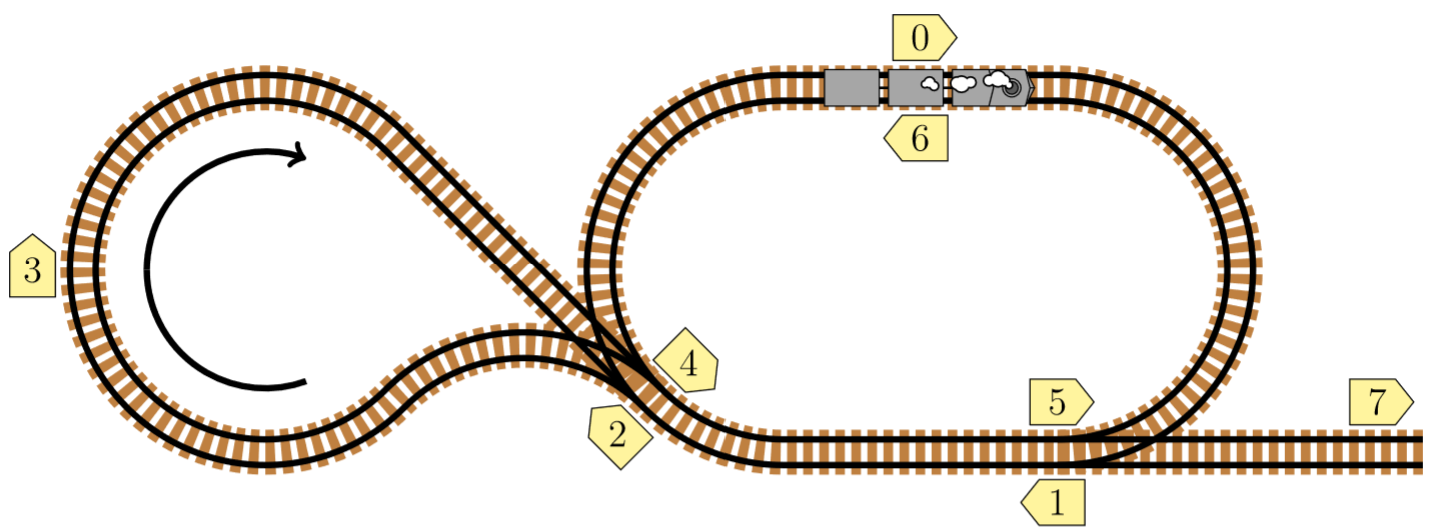
\includegraphics[scale=0.8]{fs18_t8.png}
\end{center}
\textbf{8a} Promela model for train system
\begin{verbatim}
byte pos = 0; // train position
init {
    do
        :: pos >= 0 && pos <= 5 -> pos = pos + 1
        :: pos == 2 -> pos = 0
        :: pos == 5 -> pos = 7
        :: pos == 6 -> pos = 4
        :: pos == 7 -> break; // end point
    end
}
\end{verbatim} 
\textbf{8b} \texttt{assert}-statements can be used to test \textbf{safety} properties: can check if the "bad thing" happened up to that point. For a liveness property we would have to know what happens after. \smallskip \\
\textbf{8c} For the four statements: Can you modify the promela code using assert statements to check this property? If yes, state how, if no, state why not. 
\begin{enumerate}
    \item "The train will never reach position 6": \\
    Change \texttt{::pos == 6 -> pos = 4} to \texttt{::pos == 6 -> assert (false);}
    \item "The train is guaranteed to eventually position 7":\\
    Liveness property, cannot be checked 
    \item "It is possible for the train to reach position 7": \\
    Change \texttt{::pos == 5 -> pos = 7} to \texttt{::pos == 5 -> assert (false); pos = 7;}
    \item "The train cannot reach position 7 without first visiting position 3": \\
    Add \texttt{pos == 3 -> break;}. Change \texttt{::pos == 7 -> break;} to \texttt{::pos == 7 -> assert (false);}. Change \texttt{::pos >= 0 \&\& pos <= 5 -> break;} to \texttt{::pos >= 0 \&\& pos <= 2 -> pos = pos + 1;} and  \texttt{::pos >= 4 \&\& pos <= 5 -> pos = pos + 1;}. You can't continue after visiting 3. If the assertion does not get triggered then there is no way to reach 7 without first visiting 3.
    
\end{enumerate}

\section{Linear temporal logic}
\subsection{Properties}
A \textbf{finite transition system} is a tuple $(\Gamma, \Sigma_I, \li)$
\begin{itemize}
    \item $\Gamma$: a finite set of configurations
    \item $\sigma_I\in \Gamma$: an initial congiguration
    \item $\li \subseteq \Gamma \times \Gamma$: a transition relation
    \item ommiting terminal configurations
\end{itemize} \smallskip
$\gamma \in \Gamma^\omega$ ($\Gamma^\omega$ set of infinite sequences) is a \textbf{computation} of a transition system if:
\begin{itemize}
    \item $\gamma_{[0]}=\sigma_I$
    \item $\gamma_{[i]} \li \gamma_{[i+1]}$ (for all $i \geq 0$)
\end{itemize} \smallskip
\textbf{Linear-time property $P$ over $\Gamma$}: subset of $\Gamma^\omega$ \smallskip \\
\textbf{Atomic proposition $AP$}: proposition containing no logical connectives \smallskip \\
\textbf{Labling function}: $L:\Gamma \mapsto \P(AP)$, we call $L(\sigma)$ an \textbf{abstract state} \smallskip \\
\textbf{Trace $t\in \P(AP)^\omega$}: Abstraction of a computation, $t = L(\gamma_{[0]})L(\gamma_{[1]})L(\gamma_{[2]})...$ for a transition system \smallskip \\
\textbf{Liveness property} \begin{itemize}
    \item Intuition: if the thing has not happened yet, it could happen in the future
    \item A liveness property does not rule out any prefix
    \item Every finite prefix can be extended to an infinte sequence that is in $P$
    \item Liveness properties are violated in infinite time
\end{itemize} \smallskip
\textbf{Safety property} \begin{itemize}
    \item Intuition: Something bad is never allowed to happen (and can't be fixed)
    \item If in a finite prefix a property is violated, all sequences with this prefix violate the property
    \item Liveness properties are violated in finite time
\end{itemize} \smallskip

\subsection{Operators}
For a trace $t\in\P(AP)^\omega$
\begin{center}
    \begin{tabular}{l l l}
        $t \vDash p$ & iff $p \in t_{[0]}$ & now \\
        $t \vDash\lnot \phi$ & iff not $\phi \in t_{[0]}$ & not now \\
        $t \vDash \phi \land \psi$ & iff $t \vDash \phi$ and $t \vDash \psi$ & and \\
        $t \vDash \phi \unt \psi$ & iff $\exists k \geq 0$ with  $t_{\geq k} \vDash \psi$ and $t_{\geq j} \vDash \phi$ $\forall 0 \leq j < k$ & until \\
        $t \vDash \nex \phi$ & iff  $t_{[1]} \vDash \phi$ & next \\
        $t \vDash \evt \phi$ & $\equiv true \unt \psi$ & eventually \\
        $t \vDash \alw \phi$ & iff  $\equiv \lnot (\evt (\lnot  \phi))$ & always (from now) \\
    \end{tabular}
\end{center}

\subsubsection{Sheet 13, Ex.2}
Transition system $T$  with atomic propositions $P=\{p,q,r\}$
\begin{center}
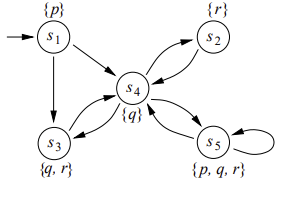
\includegraphics[scale=0.8]{sheet13_a2.png}
\end{center}
\textbf{2.1} Which of the following LTL formulas are satisfied in $T$?
\begin{itemize}
    \item $\varphi_1 = \evt \alw r$ "=" eventually always $r$: $T \nvDash \varphi_1$, counter example $\gamma = s_1s_4s_5s_4s_5s_4\dots$
    \item $\varphi_2 = \alw \evt r$ "=" always eventually $r$: $T \vDash \varphi_2$ since there is no loop in which r does not hold at some point 
    \item $\varphi_3 = \nex \lnot r \Rightarrow \nex \nex r$ "=" next not r implies second next r: $T \vDash \varphi_3$, $\lnot r$ holds in $s_4$ and $s_1$. $s_1$ cannot be reached as next state. From $s_4$ we transition to one of $s_2, s_3, s_5$, where $r$ holds
    \item $\varphi_4 = \alw p$ "=" always $p$: $T \nvDash \varphi_4$, counter example $\gamma = s_1s_4s_5s_4s_5s_4\dots$
    \item $\varphi_5 = p \unt \alw (q \lor r)$ "=" $p$ until always $q$ or $r$: after starting at $s_1$ where $p$ holds, the state changes between $s_2,s_3,s_4,s_5$, where $q \lor p$ holds 
    \item $\varphi_6 = (\nex \nex q) \unt (q \lor r)$ "=" second next $q$ until $q$ or $r$: $T \nvDash \varphi_6$, counter example $\gamma = s_1s_4s_2s_4s_2s_4\dots$
    \item $\varphi_7 = \evt \alw \nex q$ "=" eventually always $q$ as next: $T \nvDash \varphi_7$, counter example $\gamma = s_1s_4s_2s_4s_2s_4\dots$
    \item $\varphi_8 = (\evt \alw p) \Rightarrow  (\evt \alw r)$ "=" if eventually always r holds, then eventually always t holds: $(\evt \alw p)$ holds only if the trace goes into a loop $s_5s_5s_5\dots$. For those traces $\evt \alw r$ holds. If $(\evt \alw p)$ does not hold, the implication holds trivially
\end{itemize}
\textbf{2.2} Formalize the following properties in LTL
\begin{enumerate}
    \item Eventually, it will not be possible for the system to go to state $s_1$: $\evt \alw \lnot (p \land \lnot q \land \lnot r)$
    \item Whenever the system is in a state that satisfies $r$, then the next state satisfies $q$: $\alw (r \Rightarrow \nex q)$
    \item $p$ always implies $r$ except perhaps in the initial state: $\nex \alw (p \Rightarrow r)$ (possible alternative solution: $\alw(p \land (q \lor r)\Rightarrow r)$)
    \item Whenever the system is in state $s_5$, it will remain there until $r$ becomes false: $\alw ((p \land q \land r ) \Rightarrow ((p \land q \land r) \unt \lnot r) )$
    \item $q$ will be true at least twice: $\evt(q \land \nex \evt q)$
    \item $q$ will be true infinitely often: $\alw \evt q$
    \item If $p$ is true only at the initial state of a trace, then $r$ is false infinitely many times in that trace: $(p \land \nex\alw \lnot p) \Rightarrow (\alw \evt \lnot r)$
    \item $s4$ can never be repeated (there is no transition from s4 to itself): $\alw(\lnot p \land q \land \lnot r \Rightarrow \nex \lnot (\lnot p \land q \land \lnot r))$
\end{enumerate}


\end{document}

